\documentclass[../NormeProgetto.tex]{subfiles}

\begin{document}
\section{Processi organizzativi}
	\subsection{Gestione organizzativa}
	\subsubsection{Comunicazione}
		\paragraph{Comunicazioni interne}
			Per le comunicazioni interne è stato scelto di utilizzare lo strumento Messages messo a disposizione da Teamwork\g.
			La procedura per inviare un messaggio ai membri del gruppo è la seguente:
			\begin{enumerate}
				\item accedere a Teamwork\g\ ed entrare nella sezione Messages;
				\item creare un nuovo messaggio inserendo oggetto e corpo del messaggio;
				\item selezionare i destinatari del messaggio ed inviare il messaggio.
			\end{enumerate}
			Per rispondere ad un messaggio ricevuto la procedura è la seguente:
			\begin{enumerate}
				\item accedere a Teamwork\g\ ed entrare nella sezione Messages;
				\item selezionare il messaggio al quale si vuole rispondere ed inviare la risposta.
			\end{enumerate}
			 Tale sistema deve essere utilizzato solo per questioni riguardanti il progetto. \\
			Per i messaggi brevi, al fine di velocizzare le comunicazioni interne, il gruppo utilizzerà lo strumento di messaggistica Telegram\g. Inoltre, per le videochiamate, è stato scelto di utilizzare Skype\g. \\
			Qualora i sistemi sopra elencati venissero utilizzati per decisioni rilevanti per lo sviluppo del progetto è necessario stilare un verbale.\\
			I membri del gruppo sono tenuti a prestare attenzione al numero di messaggi diffusi per non creare difficoltà di comunicazione. 
		\paragraph{Comunicazioni esterne}
			Per la comunicazioni esterne è stato creato un apposito indirizzo di posta elettronica: \mailleaf. \\
			Il \responsabilediprogetto\ ha l'incarico di mantenere i contatti tra il team\g\ e le componenti esterne utilizzando tale indirizzo di posta elettronica. Inoltre è suo compito informare i membri del gruppo delle discussioni avvenute con componenti esterne: questo può essere fatto riassumendo la conversazione in una email e inviandola alla mailing list del gruppo.
		\paragraph{Composizione delle email}
			Questa sezione tratta le norme da rispettare nella composizione delle email, sia per la comunicazione interna che esterna.
			\subparagraph{Mittente}
				Nel caso di comunicazione interna il mittente dovrà essere l'indirizzo di posta elettronica personale del membro del gruppo che ha scritto l'email, mentre in caso di comunicazione esterna l'unico indirizzo che deve essere utilizzato è \mailleaf. \\ Qualora la comunicazione debba avvenire tra un numero ristretto di persone all'interno del gruppo, questi potranno utilizzare i loro indirizzi email personali.
			\subparagraph{Destinatario}
				Nel caso di comunicazione interna al gruppo l'unico destinatario deve essere \mailleaf\ per facilitare l'invio a tutti i membri del gruppo stesso, mentre in caso di comunicazione esterna il destinatari possono essere il Prof. Tullio Vardanega, il Prof. Riccardo Cardin oppure i proponenti del progetto, a seconda dello scopo dell'email.
			\subparagraph{Oggetto}
				L'oggetto dell'email deve sintetizzare il contenuto dell'email stessa in modo più chiaro ed esaustivo possibile. Possibilmente l'oggetto di una nuova email deve essere differente rispetto alle email inviate e ricevute in precedenza, in modo tale da rendere facilmente identificabile ogni messaggio. \\ Per comporre un messaggio di risposta è necessario anteporre all'oggetto il prefisso ``Re:'', mentre nel caso di inoltro di un messaggio è obbligatorio aggiungere il prefisso ``I:''. In entrambi i casi, le rimanenti parti dell'email non vanno modificate.
			\subparagraph{Corpo}
				Il corpo del messaggio deve essere esaustivo, sintetico e deve essere comprensibile a tutti i destinatari del messaggi. \\ In caso di risposta o inoltro è preferibile aggiungere la nuova parte di testo all'inizio dell'email per permettere una più facile lettura del contenuto. \\ Nell'eventualità che nel contenuto di un'email ci si debba riferire a persone è preferibile utilizzare la sintassi: ``'Nome Cognome'', nel caso invece in cui si debba fare esplicito riferimento ad un ruolo di progetto è consigliabile riportarne per intero il nome.
			\subparagraph{Allegati}
				Si consiglia di non fare uso di allegati per lo scambio di documenti o file, a meno che non sia strettamente necessario. È preferibile, invece, caricare questi file in una cartella di Google Drive\g\ e inviare per email il link al documento o file desiderato. \\ Sia in caso di invio di allegati, che di link a documenti o file è buona norma inserire una breve descrizione di presentazione dell'allegato in modo tale che sia possibile in modo semplice capire di cosa si tratta. \\ Infine si chiede di prestare attenzione al formato dei documenti e file.
	\subsubsection{Riunioni}
		Il \responsabilediprogetto\ ha il compito di indire le riunioni sia interne che esterne. Per ogni riunione il \responsabilediprogetto\ dovrà inviare un messaggio tramite l'apposito strumento messo a disposizione da Teamwork\g, con la seguente struttura:
		\begin{itemize}
			\item \textbf{oggetto}: convocazione della riunione N per il giorno AAAA-mm-GG;
			\item \textbf{corpo}: 
			\begin{itemize}
				\item data;
				\item ora;
				\item luogo;
				\item tipo di riunione;
				\item ordine del giorno.
				\end{itemize}
		\end{itemize}
		Dove N rappresenta il numero della riunione e tipo indica se la riunione sia interna richiesta dal \responsabilediprogetto, interna richiesta da uno o più dai membri del gruppo oppure esterna. \\
		Le informazioni sulle riunioni devono essere presentate con più preavviso possibile, almeno tre giorni prima in modo tale che i membri del gruppo possano organizzare i loro impegni ed essere presenti alla riunione.
		\paragraph{Riunioni interne}
			\subparagraph{Convocazione di una riunione interna}
				In generale, il compito di convocare le riunioni interne spetta al \responsabilediprogetto, che può indire le riunioni quando più lo ritiene opportuno. Gli altri componenti del gruppo possono richiedere una riunione interna straordinaria, presentando al \responsabilediprogetto\ le motivazioni per le quali si ritiene necessaria una riunione. In questi casi il \responsabilediprogetto\ può:
				\begin{itemize}
					\item autorizzare lo svolgimento della riunione;
					\item negare lo svolgimento della riunione, nel caso in cui non ritenga le motivazioni presentate valide abbastanza da richiedere una riunione;
					\item suggerire mezzi di comunicazione differenti.
				\end{itemize}
				In ogni caso spetta al \responsabilediprogetto\ decidere data, ora e luogo dell'incontro contattando i membri del team\g\ e chiedendo loro la disponibilità. Questi sono tenuti a rispondere tempestivamente in modo tale da dare la possibilità al \responsabilediprogetto\ di anticipare o posticipare la data o l'ora della riunione.
			\subparagraph{Gestione di una riunione interna}
				All'inizio di ogni riunione interna il \responsabilediprogetto\ nomina un segretario che ha il compito di redigere la minuta della riunione, catturando possibilmente tutti e soli gli aspetti più importanti della riunione stessa. Terminato l'incontro, il segretario ha il compito di redigere il verbale dell'incontro. Questo verbale verrà archiviato nel repository\g\ del gruppo, per la consultazione di tutti i membri. \\ Durante le riunioni i partecipanti devono tenere un comportamento che favorisca la discussione all'interno del gruppo e di tutti gli argomenti previsti. 
		\paragraph{Riunioni esterne}
				\subparagraph{Convocazione di una riunione esterna}
					Il \responsabilediprogetto\ ha il compito di fissare le riunioni esterne con i proponenti o con i committenti, contattandoli tramite la casella di posta elettronica del gruppo.\\ Il \responsabilediprogetto\ ha, inoltre, il compito di accordarsi con i proponenti o committenti riguardo data, orario e luogo dell'incontro, tenendo conto anche della disponibilità degli elementi del gruppo e cercando, per quanto possibile, di far partecipare tutti alla riunione.
				\subparagraph{Gestione di una riunione esterna}
					Ad ogni riunione esterna il \responsabilediprogetto\ deve chiedere la disponibilità ai proponenti o committenti di fare una registrazione audio dell'incontro. Ciò permetterà, alla fine della riunione, di redigere un verbale che sia quanto più fedele possibile a ciò di cui si è discusso durante l'incontro. In questo modo anche eventuali membri assenti alla riunione potranno disporre di un documento che riporti i temi trattati in modo esaustivo. In questo caso, come per le riunioni interne, viene nominato un segretario che ha il compito di riascoltare l'incontro e di scriverne un verbale. In caso non fosse possibile registrare l'incontro il \responsabilediprogetto\ deve redigere il verbale della riunione esterna, avvalendosi dell'aiuto di tutti i membri del team\g\ presenti all'incontro. Questo permetterà di avere una trascrizione più fedele possibile dei contenuti.
		\paragraph{Verbale di una riunione}
			Il verbale di una riunione è un documento nel quale vengono riassunti gli argomenti trattati e nel quale vengono indicate eventuali decisioni prese nel corso della riunione stessa.\\ Il compito della stesura del verbale spetta:
			\begin{itemize}
				\item ad un segretario, nominato all'inizio di una riunione interna oppure alla fine di una riunione esterna nella quale è stato dato il permesso di registrare l'incontro;
				\item al \responsabilediprogetto\ con l'aiuto di tutto il gruppo, nel caso di riunione esterna senza la possibilità di registrare quanto è stato detto.
			\end{itemize}
			I verbali dovranno avere queste struttura:
			\begin{itemize}
				\item dove e quando si è svolta la riunione;
				\item quali membri hanno partecipato alla riunione e quali membri erano, invece, assenti;
				\item il nome dell'eventuale segretario oppure del \responsabilediprogetto\ che ha redatto il verbale;
				\item tipo di riunione;
				\item ordine del giorno;
				\item eventuali argomenti dell'ordine del giorno non trattati;
				\item gli interventi più significativi in ordine temporale;
				\item suggerimenti, proposte, decisioni emerse durante la riunione;
				\item dubbi, problematiche emerse durante la riunione;
				\item eventuali compiti assegnati a membri del gruppo, con indicazione di nome, cognome e ruolo della persona a cui è stato assegnato;
				\item eventuali argomenti da trattare nella prossima riunione.
			\end{itemize}
	\subsubsection{Ruoli di progetto}
		Per lo sviluppo collaborativo del progetto, ai membri del gruppo saranno assegnati dei ruoli differenti che corrispondono a figure professionali. Ogni membro dovrà ricoprire ogni ruolo almeno una volta ed è necessario garantire che il ruolo di ciascun membro del gruppo non sia in conflitto con il ruolo che ha ricoperto in passato. È compito del \verificatore\ controllare che siano rispettate queste condizioni, in caso contrario dovrà avvertire il \responsabilediprogetto\ che dovrà risolvere il problema.
		\paragraph{Responsabile di progetto}
			Il \responsabilediprogetto\ rappresenta il progetto presso il fornitore e presso il committente, accentrando su di sé la responsabilità di scelta e approvazione. Per questo motivo ha responsabilità su:
			\begin{itemize}
				\item pianificazione, coordinamento e controllo delle attività;
				\item gestione delle risorse;
				\item analisi e gestione dei rischi;
				\item approvazione dei documenti;
				\item approvazione dell'offerta economica;
				\item convocazione delle riunioni interne;
				\item relazioni esterne;
				\item assegnazione delle attività a persone.
			\end{itemize}
			Per questi motivi ha il compito di:
			\begin{itemize}
				\item assicurarsi che le attività di verifica e validazione siano svolte seguendo le \normediprogetto;
				\item garantire il rispetto dei ruoli e dei compiti assegnati nel \pianodiprogetto.
			\end{itemize}
		\paragraph{Amministratore}
			L'\amministratore\ è responsabile del controllo e della gestione dell'ambiente di lavoro. In particolare deve preoccuparsi di:
			\begin{itemize}
				\item equipaggiare l'ambiente di lavoro con strumenti, procedure, infrastrutture e servizi a supporto dei processi che permettano di automatizzare il più possibile le attività o parti di esse;
				\item garantire che l'ambiente di lavoro sia completo, dotato di tutti gli strumenti necessari al progetto, ordinato e aggiornato;
				\item controllare le versioni e configurazioni del prodotto\g;
				\item gestire la documentazione, controllarne la diffusione, la disponibilità e l'archiviazione;
				\item fornire procedure e strumenti per il monitoraggio e segnalazione per il controllo qualità;
				\item risolvere problemi legati alla gestione dei processi tramite l'adozione di strumenti adatti.
			\end{itemize}
			L'\amministratore\ redige inoltre le \normediprogetto\, dove viene spiegato l'utilizzo degli strumenti, e deve redigere la sezione del \pianodiqualifica\ dove vengono descritti gli strumenti e i metodi atti alla verifica. L'\amministratore\ non compie scelte gestionali, ma tecnologiche concordate con il \responsabilediprogetto.
		\paragraph{Analista}
			L'\analista\ è il responsabile delle attività di analisi. Le mansioni che gli competono riguardano:
			\begin{itemize}
				\item comprendere la natura e la complessità del problema tramite l'analisi dei bisogni e delle fonti;
				\item classificare i requisiti;
				\item stendere i diagrammi dei casi d'uso;
				\item assegnare i requisiti a parti distinte del sistema;
				\item assicurarsi che i requisiti trovati siano conformi alle richieste del proponente.
			\end{itemize}
			L'\analista\ non si occupa di trovare una soluzione al problema, ma lo definisce redigendo lo \studiodifattibilita\ e l'\analisideirequisiti. Partecipa alla definizione del \pianodiqualifica\ in quanto conosce a fondo il problema e deve avere chiari i livelli di qualità richiesti, oltre alle procedure per ottenerli. 
		\paragraph{Progettista}
			Il \progettista\ è il responsabile delle attività di progettazione. I compiti a lui affidati comprendono:
			\begin{itemize}
				\item produrre una soluzione attuabile e che sia comprensibile e soddisfacente per gli stakeholders;
				\item effettuare scelte su aspetti progettuali che applichino al prodotto\g\ soluzioni note ed ottimizzate;
				\item effettuare scelte su aspetti progettuali e tecnologici che rendano il prodotto\g\ facilmente manutenibile;
				\item effettuare scelte su aspetti progettuali e tecnologici che rendano il prodotto\g\ realizzabile con costi e scadenze prefissate.
			\end{itemize}
			Il \progettista\ redige i documenti di \specificatecnica, \definizionediprodotto\ e si occupa delle sezioni del \pianodiqualifica\ relative alle metriche di verifica della programmazione.
		\paragraph{Programmatore}
			Il \programmatore\ è responsabile delle attività di codifica e delle componenti di ausilio necessarie per l'esecuzione delle prove di verifica e validazione. In particolare ha i seguenti compiti:
			\begin{itemize}
				\item implementare in maniera rigorosa le soluzioni descritte dal \progettista;
				\item scrivere codice che sia documentato, manutenibile e che rispetti le metriche stabilite per la scrittura del codice;
				\item realizzare i test per la verifica e la validazione del codice stesso;
				\item redigere il manuale per gli sviluppatori.
			\end{itemize}
			Il \programmatore, infine, deve occuparsi di redigere il \manualeutente.
		\paragraph{Verificatore}
			Il \verificatore\ è il responsabile delle attività di verifica. Le mansioni che gli competono sono:
			\begin{itemize}
				\item garantire che l'attuazione delle attività sia conforme alle norme stabilite;
				\item verificare che le attività svolte non abbiano introdotti errori;
				\item controllare la conformità di ogni stadio del ciclo di vita del prodotto\g.
			\end{itemize}
			Il \verificatore\ deve redigere le sezioni del \pianodiqualifica\ riguardanti l'esito e la completezza delle verifiche effettuate.
		\paragraph{Rotazione dei ruoli}
			Ogni membro del gruppo dovrà ricoprire ciascuno dei ruoli del progetto. La pianificazione dovrà essere redatta prestando attenzione a quanto segue:
			\begin{itemize}
				\item ogni membro del gruppo non dovrà mai ricoprire un ruolo che preveda la verifica dell'operato svolto da lui in precedenza poiché questo potrebbe portare ad un conflitto di interesse;
				\item bisogna tener conto dei possibili impegni o interessi dei singoli membri del gruppo;
				\item ciascun membro dovrà assicurare l'esclusivo svolgimento del ruolo a lui assegnato.
			\end{itemize}				
	\subsubsection{Ticketing}
			I ticket\g\ rappresentano l'associazione tra un membro del gruppo ed una attività. Lo strumento scelto per la loro creazione e gestione è Teamwork\g (vedi sezione \hyperref[sec: Pianificazione Teamwork]{Pianificazione}). Per ogni ticket\g\ valgono le seguenti norme:
			\begin{itemize}
				\item possono essere creati solamente dal \responsabilediprogetto;
				\item alla creazione di un nuovo ticket\g, l'assegnatario deve esserne informato;
				\item è consigliabile che non vi siano più di 3 ticket\g\ per ogni attività. Nel caso in cui questo dovesse accadere, il \responsabilediprogetto\ dovrebbe valutare la possibilità di suddividere l'attività in sotto-attività più piccole, ciascuna delle quali realizzabile da un sola persona.
			\end{itemize}			 
			 È consigliabile che i membri del gruppo accedano quotidianamente a Teamwork\g\ per verificare quali siano i ticket\g\ a loro assegnati e riportare lo stato di avanzamento dell'attività a loro assegnata.

		\subsubsection{Procedure}
			\paragraph{Procedura di creazione e gestione di un ticket}
				Per la creazione di un nuovo ticket\g\ il \responsabilediprogetto, deve accedere a Teamwork\g\ ed entrare nella sezione Tasks. Ogni task sarà associato ad una Task List, per cui nel caso non fosse presente dovrà essere creata. La procedura per la creazione di un task è la seguente:
				\begin{enumerate}
					\item il \responsabilediprogetto\ crea un nuovo task;
					\item nel caso in cui il task fosse fuori dalla portata di un singolo membro del gruppo, può suddividerlo il sotto-task, se ha le conoscenze per farlo;
					\item i task e i sotto-task vengono assegnati ai membri del gruppo;
					\item l'assegnatario del task può a sua volta suddividerlo in sotto-task per organizzare meglio l'attività, assegnandoli a se stesso e dotandoli di titolo e descrizione esplicativa, inserendovi le azioni per portare a termine il task sotto forma di checklist, in cui ogni azione corrisponde ad una checkbox \texttt{- [ ]}.
				\end{enumerate}
				\begin{figure}[H]
					\centering
					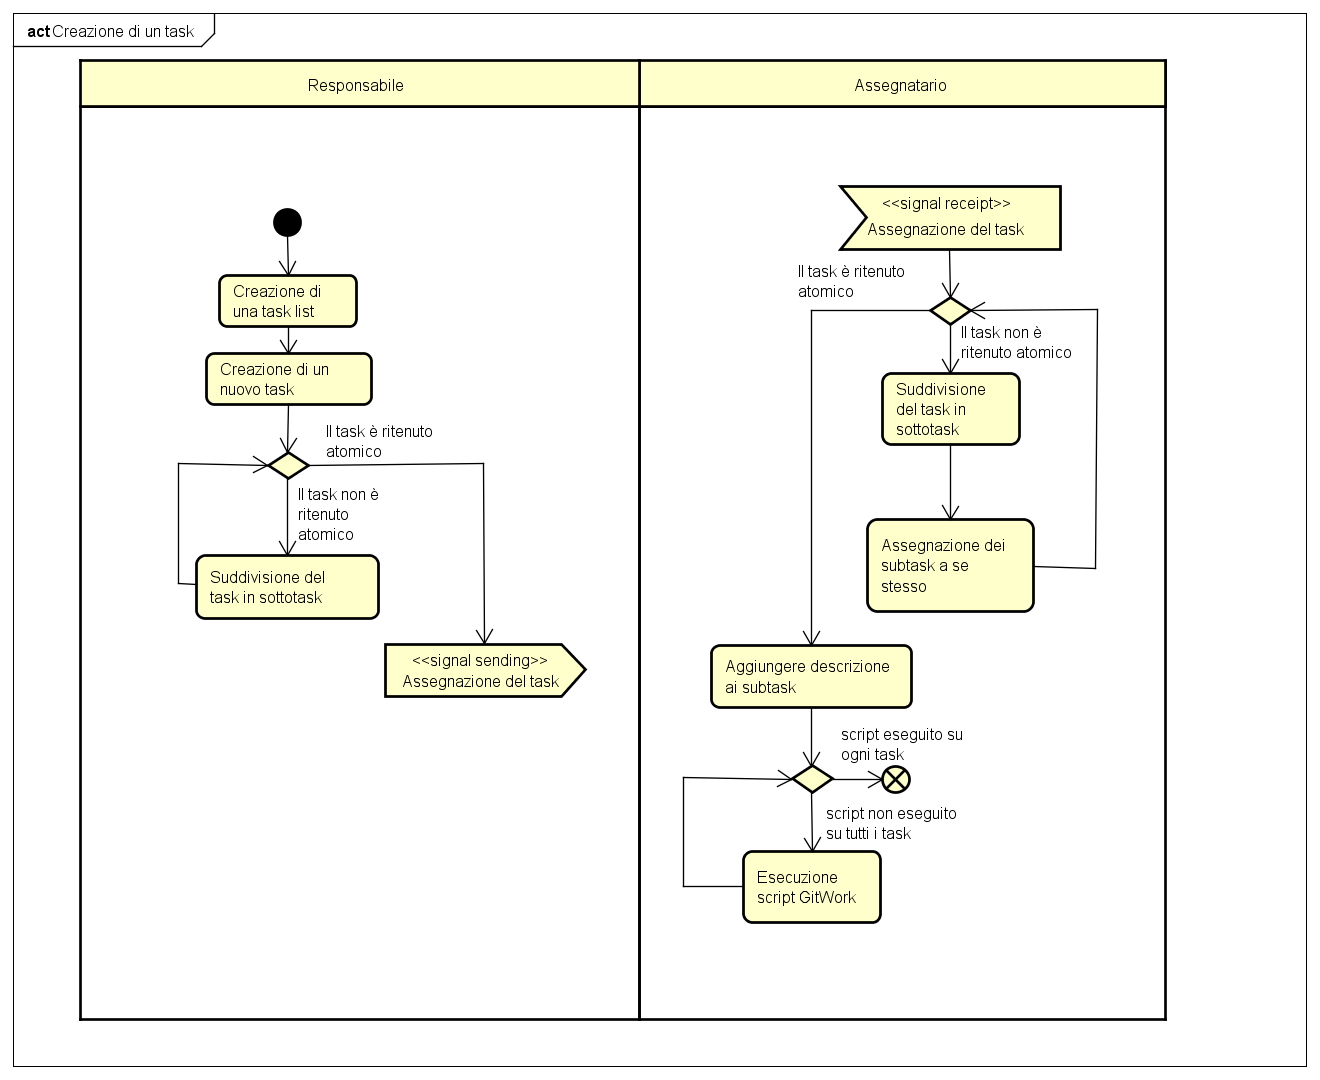
\includegraphics[scale=0.55]{sections/img/creazioneTask.png}
					\caption{Procedura di creazione e gestione di un ticket}\label{fig:Procedura di creazione e gestione di un ticket - Parte 1} 
				\end{figure}
			Una volta creato il ticket su Teamwork, i passi da seguire sono i seguenti			
				\begin{enumerate}
					\item per ogni task aperto aperto al punto 1, l'assegnatario del task esegue lo script \textit{GitWork.java} che creerà, sul repository del gruppo \leaf\ una issue per ogni subtask del task selezionato, con la label ToDo;
					\item quando il membro del gruppo inizierà effettivamente a lavorare sulla issue, modificherà la label da ToDo a Working;
					\item ogni commit eseguito dovrà riferirsi ad una delle issue presenti sul repository, mediante \texttt{\# numeroIssue} all'interno del messaggio di commit. Inoltre, sarà necessario spuntare la relativa checkbox per indicare l'avanzamento del proprio lavoro;
					\item completato il lavoro, inserire nel messaggio di commit la stringa \texttt{£toVerify} in modo che la label della issue venga modificata da ToDo a toVerify.
				\end{enumerate}
			A questo punto, è possibile verificare la issue e, di conseguenza, il ticket.
				\begin{figure}[H]
					\centering
					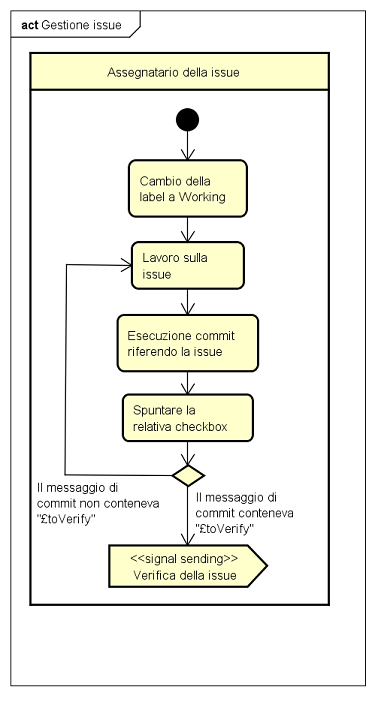
\includegraphics[scale=0.5, width=\textwidth]{sections/img/lavoroSuIssue.png}
					\caption{Procedura di creazione e gestione di un ticket}\label{fig:Procedura di creazione e gestione di un ticket - Parte 2} 
				\end{figure}
		\subsubsection{Strumenti}
			\paragraph{Pianificazione} \label{sec: Pianificazione Teamwork}
				Lo strumento scelto per la gestione delle attività di pianificazione di progetto è Teamwork\g. Le caratteristiche rilevanti di questo software\g\ sono le seguenti:
				\begin{itemize}
					\item creazione di attività e sotto-attività assegnabili ad uno o più membri del progetto;
					\item possibilità di creare dipendenze tra le attività;
					\item possibilità di assegnare priorità differenti ad ogni attività;
					\item creazione di milestones da impostare sul calendario;
					\item creazione automatica di grafici e report, tra cui il diagramma di Gantt;
					\item dashboard\g\ che permette di aver un riepilogo dello stato di avanzamento del progetto, con segnalazione di eventuali ritardi;
					\item strumento per la segnalazione dei rischi;
					\item sistema di gestione delle notifiche per ogni attività svolta;
					\item versione mobile;
				\end{itemize}		 
				Questo strumento, dopo essere stato valutato insieme ad altri strumenti quali Trello, Freedcamp\g\ e Zoho, è risultato essere il più completo.
			
			\paragraph{Creazione dei diagrammi di Gantt}
				Lo strumento scelto per la realizzazione dei diagrammi di Gantt\g\ è GanttProject. Le principali ragioni per cui è stato scelto sono:
				\begin{itemize}
					\item gratuito;
					\item open source\g;
					\item multipiattaforma;
					\item compatibile con i diagrammi generati da Teamwork\g;
					\item offre la possibilità di creare i diagrammi PERT\g;
					\item offre la possibilità di creare grafici di WBS\g;
					\item generazione dei diagrammi nei formati PDF\g, PNG\g, HTML\g.
				\end{itemize}
	\subsection{Formazione}
		\subsection{Ore rendicontabili e non rendicontabili}
			Aggiungere norma per rendicontare le ore.			
\end{document}
